\chapter{Graph comparison \label{ch:gc}}

Graph comparison may be reduced to a problem of measuring the difference 
between two graphs. 
A primary goal of the visualization system is to allow the user to better 
verify their numerical results with visual intuition. As such, the graph 
comparison measure is an important output of the VS that allows the user to 
quantify the difference between the methods, prompting the user to rethink 
their methods as needed. Furthermore, graph comparison may be directly used to 
compare visual and numeric correlation graphs, which we utilize to select 
stocks for a portfolio in Chapter~\ref{ch:usage}.

\section{Graph summarization}
\label{sec:gc:litreview}

There are two ways of thinking about graph comparison. Let 
$\hat{G^1}=(V^1,E^1)$ and $\hat{G^2}=(V^2,E^2)$ each be some labeled graph. 

\tablespacing
\begin{enumerate}
	\item \textbf{Graph summarization:} Compute some vector 
	$v^1$ on $\hat{G^1}$ that ``summarizes'' various properties that
	it has. Similarly, compute $v^2$ on $\hat{G^2}$ to capture 
	the same properties that $v^1$ does. Finally, compute 
	$f(v^1,v^2)$ where $f$ is some distance 
	function (e.g. Euclidean distance). A high value indicates strong 
	dissimilarity while a low value indicates similarity. 
	
	\item \textbf{Graph distance:} Create a valid distance function $f$ on the 
	graphs $\hat{G^1}, \hat{G^2}$ directly rather than a vector of metrics 
	($v^1,v^2$). 
	Compute $f(\hat{G^1},\hat{G^2})$. Again, a high value indicates strong 
	dissimilarity while a low value indicates similarity. The \textit{random 
	walk kernel} is one such example of a graph distance 
	metric~\cite{vishwanathan2010}.
\end{enumerate}
\bodyspacing

We specifically focus on the graph summarization comparison because it 
fulfills both desired criteria for the visualization system; an understanding 
of each summarization method allows the user to gain intuition on the qualities 
of the graph, and the difference between two graph summarization methods can be 
quantified easily. To be more specific, we seek to better understand the 
qualities of existing graph summarization methods and their associated 
advantages and disadvantages. 
Understanding these metrics is important due to the complex nature of graphs.
It is natural to ask why we cannot just plot the graphs instead (which are 
typically in the form of either an adjacency matrix of list of edges) and 
examine the result for visual patterns in order to understand the qualities 
of the graph. This is unfeasible for several reasons (see 
Figure~\ref{fig:gc:arr_density}). 

\tablespacing
\begin{itemize}
	\item \textbf{Arrangement:} Different arrangements of nodes on the visual 
	plane may have a profound effect on the interpretability of the graph; from 
	the start, it is unclear what the best arrangement might be, and it is 
	unfeasible for an analyst to try all possible arrangements 
	especially as the number of variables increase.
	
	\item \textbf{Density:} The more nodes there are, the more edges there may 
	be, and the more dense a graph may become, making it incredibly difficult 
	to interpret. Furthermore, it makes it more difficult to find anomalies 
	among the variable's relationships (represented by edges). A non-existent 
	edge in a dense graph is just as important as an existent edge in a sparse 
	graph because each indicates a relationship which isn't quite like all the 
	others.
\end{itemize}
\bodyspacing

\begin{figure}[htb]
	\begin{center}
		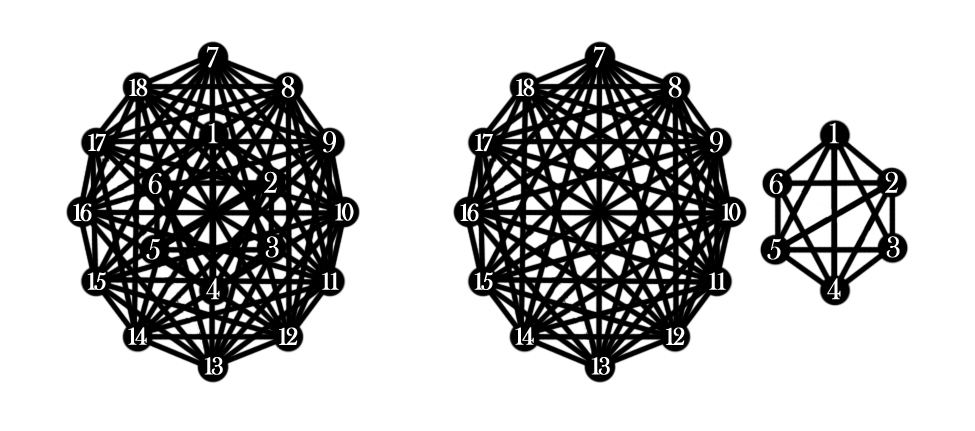
\includegraphics[width=1\linewidth]{ch-gc/figures/arr_density}
		\caption[Difficulties with graph visualization.]{
		Suppose we have a graph $G=(V,E)$ with clusters $C^1,C^2$ and $|V|=18$. 
		Let $C^1$ be composed of nodes $(V_1,...,V_6)$, and $C^2$ be composed 
		of nodes $(V_7,...,V_{18})$. 
		\textit{Left:} $C^1$, the smaller cluster, has been placed inside 
		$C^2$, the larger cluster. It is difficult to discern any meaningful 
		patterns; each node appears to be connected to every other node as the 
		density of the cluster $C^2$ makes it almost impossible to see that of 
		$C^1$.
		\textit{Right:} The nodes have been rearranged in a manner that clearly 
		distinguishes between $C^1$ and $C^2$. At a glance, it is evident that 
		$C^1$ is missing $E_{3,6}$. It is difficult to tell, however, that 
		$C^2$ is even missing an edge $(E_{13,17})$ in the first place!
		$C^1$ is more sparse, which makes it easier to visually perceive 
		anomalies in the graph.}
		\label{fig:gc:arr_density}
	\end{center}
\end{figure}

Graph summarization acts as a proxy for visually exploring the graph 
itself. Each metric, which is associated with a different characteristic of the 
graph, can be parsed and later combined to 
``reconstruct'' or better understand the qualities of each graph, subsequently 
allowing the user to better understand \textit{exactly where} the visual and 
numeric graphs differ (should the final graph comparison metric suggest that 
the two graphs are highly different). Graph distance functions skip that 
critical step by going through 
the graphs directly.

To put it in another way, graph summarization has the \textit{exact opposite 
problem} that is present in data analytics as it is practiced today (discussed 
in Chapter~\ref{ch:intro}, this is the motivation behind the VS and this 
thesis). 
The visualization system allows the user to use the visual qualities of pairwise
scatter plots to better understand numerical qualities of the data, but graph 
summarization allows the user to use numerical qualities to better understand 
the visual qualities of a graph. 

With an understanding of the properties of various graph summarization methods, 
the graph summarization difference metric may be more informative. In the VS, 
the graph summarization difference computes a list of graph summarization 
metrics $(m^\text{num},m^\text{vis})$ for each graph in order to provide a 
single vector $d$ that quantifies the difference between them with 
some difference function (e.g. Euclidean distance, L2, etc.). 
As such, a natural byproduct of the computation is 
$(m^\text{num},m^\text{vis})$, which (armed 
with an understanding of the values) provides insight on the qualities of the 
visual graph and numerical graph \textit{on an individual level} and where 
exactly their differences and similarities lie.
\section{Overview of graph summarization methods}
\label{sec:gc:methods}

\subsection{Centrality}

\subsection{Community}

\subsection{Distance matrix}

\subsection{Assortativity}

\subsection{Edge density}

\subsection{Edge connectivity}
\section{Examples}
\label{sec:gc:examples}

Table summarization of method outputs when applied to various examples we've 
thought of previously